
\chapter{闭嵌入及相关观念}
\label{ch:closed-embeddings}

\trClosedSubset{}的概形论类似物，比起\trOpenSet{}的类似物（\trOpenSubscheme/\trOpenEmbedding）来，风味出人意料地不同。然而，正如\trOpenSubscheme（\trOpenSet{}的概形论版本）局部上以\trOpenSet{} $U\subset Y$ 为模型，\trClosedSubset{}的类似物也有一个局部模型。我们对「$\Spec B$ 的\trClosedSubset{}大致对应于\trIdeal」的理解早已预示了这一点：若 $I\subset B$ 是一个\trIdeal，则 $\Spec B/I\hookrightarrow\Spec B$ 是一个\trScheme{}的\trMorphism，而且我们已经核验过：在\trTopologicalSpace{}的层面上，它把 $\Spec B/I$ 描述成 $\Spec B$ 的一个\trClosedSubset，带\trSubspaceTopology（\cref{ex:subspace-topology-inclusions}）。这个\trMorphism{}就是我们关于\trClosedSubscheme/\trClosedEmbedding{}的「局部模型」。


\section{闭嵌入与闭子概形}

\textbf{9.1.1.}\ \emph{\trhDefinition{}。}\quad 概形之间的\trMorphism{} $\pi\colon X\to Y$ 称为\textbf{\trClosedEmbedding}（closed embedding；或\textbf{\trClosedImmersion}，closed immersion），若它是一个\trAffine\trMorphism，并且对 $Y$ 的每个\trAffine\trOpenSubset{} $\Spec B\subset Y$，只要 $\pi^{-1}(\Spec B)\cong\Spec A$，映射 $B\to A$ 就都是\trSurjectiveMap{}（也就是说，形如 $B\to B/I$——我们心仪的那个局部模型）。（「嵌入」比「浸入」更可取，因为微分几何中的浸入观念，更接近代数几何学家所称的非分歧（unramified），我们将在 \S21.7 中给出它的定义。）符号 $\hookrightarrow$ 常被用来表示一个态射是\trClosedEmbedding{}（或更一般地，是\trLocally\trClosedEmbedding，见 \S9.2）。

若 $X$ 是 $Y$ 的一个\emph{子集}（且 $\pi$ 在集合的层面上就是包含映射），我们就说 $X$ 是 $Y$ 的一个\textbf{\trClosedSubscheme}。一个\trClosedEmbedding{}与「向一个\trClosedSubscheme{}的\trIsomorphism」是一回事。

\textbf{9.1.A.（练习）}\quad 证明：一个\trClosedEmbedding{}把 $X$ 的底拓扑空间与 $Y$ 的底拓扑空间的一个\trClosedSubset{}等同起来。（\trhCaveat{}：两道\trClosedEmbedding{} $\Spec k[x]/(x)\hookrightarrow\Spec k[x]$ 与 $\Spec k[x]/(x^2)\hookrightarrow\Spec k[x]$ 表明，\trClosedSubset{}并不能决定\trClosedSubscheme：那些「无穷小」的信息——或者说「绒毛」——丢失了。）

\textbf{9.1.B.（容易的练习）}\quad 证明：\trClosedEmbedding{}都是\trFinite\trMorphism，从而是\trFiniteType{}的。

\textbf{9.1.C.（容易的练习）}\quad 证明：两个\trClosedEmbedding{}的\trComposition{}仍是一个\trClosedEmbedding。

\textbf{9.1.D.（练习）}\quad 证明：「是\trClosedEmbedding」这一性质是对目标仿射局部的。

特别地，若 $B\to A$ 是环之间的一个\trSurjectiveMap，则由之诱导的\trMorphism{} $\Spec A\to\Spec B$ 是一个\trClosedEmbedding。

\textbf{9.1.2.\ 重要：\trClosedSubscheme{}对应于\trQC{}的\trIdealSheaf{}。}\quad 我们把 $\OO_Y$ 的一个 $\OO_Y$-\trSubmodule{}称为 $Y$ 上的一个\textbf{\trIdealSheaf{}}（ideal sheaf，或 sheaf of ideals）。%
一个\trClosedSubscheme{} $\pi\colon X\hookrightarrow Y$ 给出 $\OO_Y$-\trModule{}的一个\trSurjectiveMap{} $\OO_Y\to\pi_*\OO_X$。该映射的\trKernel{} $\scr{I}_{X/Y}$ 便是 $Y$ 上的一个\trIdealSheaf{}。在每个\trOpenSubset{} $\mathsf{U}$ 上，它给出环 $\OO_Y(\mathsf{U})$ 的一个理想 $\scr{I}_{X/Y}(\mathsf{U})$；而在仿射开子集 $\Spec B$ 上，它给出 $B$ 的理想 $I$，即「\trClosedSubscheme」的定义中决定满射 $B\to A=B/I$ 的那个理想。

\textbf{9.1.E.（练习）}\quad 证明：$\pi_*\OO_X$ 是 $Y$ 上的一个\trQCSheaf{}。（一条可行的进路是用\mbox{练习~6.2.D}。）

\trQCSheaf{}构成一个\trAbelianCategory，故 $\scr{I}_{X/Y}=\ker(\OO_Y\to\pi_*\OO_X)$ 也是 $Y$ 上的一个\trQCSheaf。于是，$Y$ 的每个\trClosedSubscheme{}都给出 $Y$ 上一个\emph{拟凝聚的}\trIdealSheaf{}。我们把（$Y$ 上诸拟凝聚层之间的）正合列
\begin{equation*}\tag{9.1.2.1}\label{eq:closed-subscheme-exact-sequence}
0\longrightarrow\scr{I}_{X/Y}\longrightarrow\OO_Y\longrightarrow\pi_*\OO_X\longrightarrow 0
\end{equation*}
称为 $\pi\colon X\hookrightarrow Y$ 的\textbf{闭子概形正合列}（closed subscheme exact sequence）。

我们可以经由 \eqref{eq:closed-subscheme-exact-sequence} 从\trIdealSheaf{} $\scr{I}_{X/Y}$ 把 $X$（连同它到 $Y$ 的映射 $\pi$）恢复出来：对 $Y$ 的每个仿射开子集 $\Spec B\subset Y$，在 $\Spec B$ 上取\trSection{}便给出正合列
\[
0\longrightarrow I\longrightarrow B\longrightarrow B/I\longrightarrow 0,
\]
而 $\Spec B/I$ 正是 $\pi^{-1}(\Spec B)$。

逆命题成立：

\textbf{9.1.F.（重要练习）}\quad 证明：$Y$ 上每一个拟凝聚的\trIdealSheaf{}都以这种方式产生 $Y$ 的一个\trClosedSubscheme。

这是一道很难的练习，所以作为提示，这里给出两种不同的做法；把二者以某种方式结合起来，或许正合你的心意。\emph{做法一}。对每个仿射开集 $\Spec B$，我们有\trClosedSubscheme{} $\Spec B/I(B)\hookrightarrow\Spec B$。(i) 对任意两个仿射开子概形 $\Spec A$ 与 $\Spec B$，证明：两个\trClosedSubscheme{} $\Spec A/I(A)\hookrightarrow\Spec A$ 与 $\Spec B/I(B)\hookrightarrow\Spec B$ 限制到二者的交上，给出\emph{同一个}\trClosedSubscheme。（提示：用在两个仿射开集中同时特异的开集去覆盖二者的交，命题~5.3.1。）于是，举例来说，我们便可以把这两个\trClosedSubscheme{}粘合起来，得到 $\Spec A\cup\Spec B$ 的一个\trClosedSubscheme。(ii) 用关于粘合概形的\cref{ex:glue-arbitrary-schemes}（或其中的想法），把一切仿射开子概形中的\trClosedEmbedding{}同时粘合起来。你只需要操心三重交。\emph{做法二}。(i) 先把 $X$ 描述为 $Y$ 的一个子集。(ii) 检验 $X$ 是闭的。(iii) 在这个子集上定义函数层 $\OO_X$，或许会用到\trCompatibleGerm。(iv) 检验：这样得到的\trRingedSpace{}在局部上确实就是 $\Spec B/I\hookrightarrow\Spec B$ 给出的那个\trClosedSubscheme。

\textbf{9.1.G.（不重要练习：一个作为 $\OO$-模、却不\trQC{}的\trIdealSheaf{}）}\quad 设 $X=\Spec k[x]_{(x)}$，即「仿射直线在原点处的芽」，它有两个点：一个\trClosedPoint{}与一个\trGenericPoint{} $\eta$。定义 $\scr{I}(X)=\{0\}\subset\OO_X(X)=k[x]_{(x)}$ 与 $\scr{I}(\eta)=k(x)=\OO_X(\eta)$。证明：这个\trIdealSheaf{}并不对应于任何\trClosedSubscheme。

\textbf{9.1.H.}\ \extrahard\ \textbf{（困难的（而且坦白说不重要的）练习；后文不再用到）}\quad 文献中，\trClosedEmbedding{}的惯常定义是这样一个\trMorphism{} $\pi\colon X\to Y$：$\pi$ 诱导 $X$ 的底拓扑空间到 $Y$ 的底拓扑空间之某个\trClosedSubset{}上的一个\trHomeomorphism，而且 $Y$ 上诸\trSheaf{}之间由之诱导的映射 $\pi^{\sharp}\colon\OO_Y\to\pi_*\OO_X$ 是满的。（这里说「满」，指的是诸\trStalk{}上的\trRingMorphism{}是\trSurjectiveMap。）证明：这个定义与上面给出的定义相合。（要证明我们这条涉及「在仿射开集的层面上满」的定义蕴含这个定义，你可以使用「层的态射的满性可以在适当选取的\trBase{}上检验」这一事实，\cref{ex:surjectivity-on-base}。）

至此，我们已在概形的国度里定义了开子集与闭子集的类似物。\footnote{译注：「概形的国度」（the land of schemes）是作者的惯用戏语，即「概形的世界」。}它们的定义比起经典拓扑背景中的定义来，稍微不那么「对称」：一个\trClosedSubscheme{}的「\trComplement」是唯一的一个\trOpenSubscheme，但一般地，对一个给定的\trOpenSubscheme，却有许多「互补的」\trClosedSubscheme。（我们很快就会定义其中「最好的」那一个：带\trReduced{}结构的那个，\S9.4.9。）

\textbf{9.1.3.\ 例子与性质。}

\vkexsync{I}
\begin{exercise}[重要练习]\label{ex:scheme-theoretic-union-intersection}
\begin{enumerate}[label=(\alph*)]
\item 类比闭子集，定义 $X$ 的\textbf{闭子概形的有限（\trSchemeTheoretic{}）并}（finite (scheme-theoretic) union of closed subschemes）这一观念，以及任意的（不必有限的）\textbf{闭子概形的（\trSchemeTheoretic{}）交}（(scheme-theoretic) intersection of closed subschemes）。（\mbox{练习~9.1.F} 或有帮助。）提示：若 $X$ 仿射，那么你大概会指望：对应于 $I_1$ 与 $I_2$ 的两个\trClosedSubscheme{}之并，应当是对应于 $I_1\cap I_2$ 或 $I_1I_2$ 的那个\trClosedSubscheme——但究竟是哪一个？我们会希望一个\trClosedSubscheme{}与自身之并\emph{就是}它自身，所以正确的选择是 $I_1\cap I_2$。
\item 描述 $\mathbb{A}^2$ 中 $V(y-x^2)$ 与 $V(y)$ 的\trSchemeTheoretic{}交。图~\ref{fig:scheme-theoretic-intersection} 是一幅图。（比如说，请非正式地解释：这如何对应于两条曲线在单个点处以重数 $2$ 相交——注意在你的答案里那个 $2$ 是如何显现的。或者换个问法：非既约性就这个交向你泄露了什么——既是它的「大小」，也是它的「方向」？）再描述它们的\trSchemeTheoretic{}并。
\item 证明：\trClosedSubscheme{}的有限并的底集合，就是诸底集合的有限并；对任意交亦然。
\item 描述 $\mathbb{A}^2$ 中 $V(y^2-x^2)$ 与 $V(y)$ 的\trSchemeTheoretic{}交。画一幅图。（你先前料想这个交的重数是 $1$ 还是 $2$？）由此证明：若 $X$、$Y$、$Z$ 是 $W$ 的\trClosedSubscheme，则一般地 $(X\cap Z)\cup(Y\cap Z)\neq(X\cup Y)\cap Z$。特别地，并非交与并的一切性质都能从集合搬到概形上来。
\end{enumerate}
\end{exercise}

\textbf{9.1.J.（练习）}\quad 证明：\trClosedEmbedding{}（像\trOpenEmbedding{}一样；见容易的\cref{ex:open-embeddings-are-monomorphisms}）是\trMonomorphism。

在许多情形，先验地只是闭集的那些\trLocus，常常会有作为\trClosedSubscheme{}的「\trEnrichment{}」版本（enriched versions）。%
其余的练习就是这方面的例子。（如 \S6.6.33 所描述，我们常常通过添加形容词「\trSchemeTheoretic{}的」（scheme-theoretic）来表明：我们考虑的是\trSchemeTheoretic{}的\trEnrichment{}（scheme-theoretic enrichments）——比如说，我们会说「\trSchemeTheoretic{}交」「\trSchemeTheoretic{}并」，等等。）

\vkexsync{K}
\begin{exercise}[重要练习／定义：消失概形（参看\cref{ex:vanishing-scheme-definition}）]\label{ex:vanishing-scheme-global-section}
\begin{enumerate}[label=(\alph*)]
\item 设 $Y$ 是一个\trScheme，而 $s\in\Gamma(Y,\OO_Y)$。定义由 $s$ \textbf{切出}的那个\trClosedSubscheme。我们称之为 $s$ 的\textbf{\trVanishingScheme} $V(s)$，因为它是我们早先的（集合论版本的）$V(s)$ 的\trSchemeTheoretic{}版本（\S3.4.1）。（提示：在仿射开集 $\Spec B$ 上，我们径取 $\Spec B/(s_B)$，其中 $s_B$ 是 $s$ 限制到 $\Spec B$ 上的\trSection。用\mbox{练习~9.1.F} 证明：这给出一个\trWellDefined{}的\trClosedSubscheme。）
\item 若 $u$ 是一个可逆函数，证明：$V(s)=V(su)$。
\item 若 $S$ 是一个由函数组成的集合，定义 $V(S)$。
\end{enumerate}
\end{exercise}

\textbf{9.1.4.}\ \emph{\trhDefinition{}：\trSchemeTheoretic{}支撑。}\quad 若 $M$ 是一个 $A$-\trModule，而 $\mathrm{m}\in M$，我们称 $\Spec A$ 的闭子概形 $\Spec(A/\operatorname{Ann}\mathrm{m})$ 为 $\mathrm{m}$ 的\textbf{\trSchemeTheoretic{}支撑}（scheme-theoretic support）。%
（这常被描述为「$\mathrm{m}$ 在其上有定义的最小\trClosedSubscheme」。你能把这句话讲精确吗？）

\textbf{9.1.L.（练习）}\quad 证明：$\mathrm{m}$ 的\trSchemeTheoretic{}支撑的底集合，就是通常的「集合论」支撑 $\Supp\mathrm{m}$。

\textbf{9.1.M.（练习）}\quad 把有限生成 $A$-模 $M$ 的\textbf{\trSchemeTheoretic{}支撑}（scheme-theoretic support of a finitely generated $A$-module）定义为：使 $M$ 成为一个 $(A/I)$-\trModule{}的\emph{一切}\trClosedSubscheme{} $\Spec A/I\hookrightarrow\Spec A$ 的\trSchemeTheoretic{}交。证明：它等于 $M$ 的任意一组有限生成元中诸元的\trSchemeTheoretic{}支撑的\trSchemeTheoretic{}并。

\textbf{9.1.N.（练习：把上一道练习整体化）}\quad 设 $X$ 是一个\trScheme，而 $\scr{F}$ 是 $X$ 上一个\trFiniteType{}的\trQCSheaf。你将如何定义 $\scr{F}$ 的\textbf{\trSchemeTheoretic{}支撑}？


\section{局部闭嵌入与局部闭子概形}

既然已经定义了开子集与闭子集的类似物，自然而然就该定义局部闭子集的类似物了。回想：局部闭子集是开子集与闭子集的交。因此它们是开子集的闭子集，或者等价地，是闭子集的开子集。这些等价性在概形的国度里将会有一点麻烦。（类似地，子群与商群这两个观念也不太互补。设问：群 $G$ 的「\trSubquotient」应当定义为 $G$ 的商的\trSubgroup，还是 $G$ 的\trSubgroup{}的\trQuotient？抑或二者是同一回事？在定义\trLocally\trClosedEmbedding{}时，我们将会正面撞上同一个问题。）

我们称一个\trMorphism{} $\pi\colon X\to Y$ 是\textbf{\trLocally\trClosedEmbedding}（locally closed embedding；或\textbf{\trLocally\trClosedImmersion}，locally closed immersion），若 $\pi$ 可以分解为
\[
X\xhookrightarrow[\text{\trClosed}]{\ \rho\ } Z\xhookrightarrow[\text{\trOpen}]{\ \tau\ } Y,
\]
其中（正如所标注的那样）$\rho$ 是一个\trClosedEmbedding，而 $\tau$ 是一个\trOpenEmbedding。例如，由 $(x,y)\mapsto(t,0)$ 给出的\trMorphism{} $\Spec k[t,t^{-1}]\to\Spec k[x,y]$ 就是一个\trLocally\trClosedEmbedding（图~\ref{fig:locally-closed-embedding}）。符号 $\hookrightarrow$ 常被用来表示一个态射是\trLocally\trClosedEmbedding。由于\trClosedEmbedding{}与\trOpenEmbedding{}都是\trMonomorphism（分别是练习~9.1.J 与\cref{ex:open-embeddings-are-monomorphisms}），而\trMonomorphism{}对\trComposition{}保持，所以\trLocally\trClosedEmbedding{}也是\trMonomorphism。

\begin{figure}[htbp]
\centering
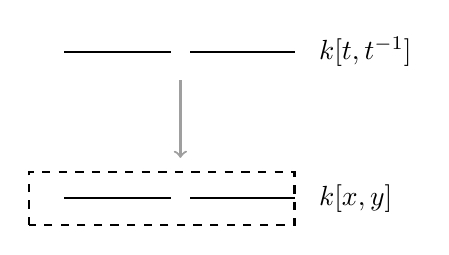
\begin{tikzpicture}[scale=0.9,line width=0.8pt]
  \draw (0,2.55) -- (1.50,2.55);
  \draw (1.78,2.55) -- (3.25,2.55);
  \node[anchor=west] at (3.45,2.55) {$\Spec k[t,t^{-1}]$};
  \draw[gray!75,->] (1.64,2.15) -- (1.64,1.05);
  \draw[dashed] (-0.50,0.10) rectangle (3.25,0.85);
  \draw (0,0.48) -- (1.50,0.48);
  \draw (1.78,0.48) -- (3.25,0.48);
  \node[anchor=west] at (3.45,0.48) {$\Spec k[x,y]$};
\end{tikzpicture}
\caption{局部闭嵌入 $\Spec k[t,t^{-1}]\to\Spec k[x,y]$（$t\mapsto(t,0)=(x,y)$，亦即 $(x,y)\mapsto(t,0)$）。（依原书手绘图重绘。）}\label{fig:locally-closed-embedding}
\end{figure}

（警告：术语\emph{浸入}常被用来指\emph{\trLocally\trClosedEmbedding}或\emph{\trLocally\trClosedImmersion}，但这是不明智的术语——理由在定义~9.1.1 处谈\trClosedEmbedding{}时就已出现：微分几何中的浸入观念，更接近代数几何学家所称的\trUnramified，我们将在 \S21.7 中给出它的定义。此外，光杆的术语\emph{嵌入}也应当避免，因为它不必要地不精确。）

\textbf{9.2.1.}\quad 若 $X$ 是 $Y$ 的一个子集（且 $\pi$ 在集合的层面上就是包含映射），我们就说 $X$ 是 $Y$ 的一个\textbf{\trLocally\trClosedSubscheme}。（警告：光杆的术语\textbf{\trSubscheme}常被用来意指\emph{\trLocally\trClosedSubscheme}，但我们将避免这种令人不快的用法。）

\textbf{9.2.A.（容易的练习）}\quad 证明：\trLocally\trClosedEmbedding{}都\trLocally\trFiniteType。

\textbf{9.2.B.（练习）}\quad 设 $\pi\colon X\to Y$ 是一个\trLocally\trClosedEmbedding，其像为 $Y$ 的一个\trClosedSubset。证明：$\pi$ 是一个\trClosedEmbedding。一条可能的提示：「是\trClosedEmbedding」这一性质是对目标仿射局部的，练习~9.1.D。（这在哲理上是很有用的；例如见 \S11.2.2。）

写到这里，你其实可以顺手定义概形 $X$ 中两个\trLocally\trClosedEmbedding{}的交（它也将是 $X$ 中的一个\trLocally\trClosedEmbedding）。但这会相当别扭，因为你将不得不证明：你的构造不依赖于每个\trLocally\trClosedEmbedding{}之分解为一个\trClosedEmbedding{}与一个\trOpenEmbedding{}时的具体方式。我们不如按兵不动，且等到\mbox{练习~10.2.C}——届时，把交认作一个\trFiberProduct{}将会使这件事容易得多。

显然，$X$ 的一个\trClosedSubscheme{} $V$ 的\trOpenSubscheme{} $U$ 可以解读为某个\trOpenSubscheme{}的\trClosedSubscheme：由于 $V$ 上的拓扑是从 $X$ 的拓扑诱导而来的，$U$ 的底集合是 $X$ 的某个\trOpenSubset{} $U'$ 与 $V$ 的交。我们可以取 $V'=V\cap U'$，于是 $V'\hookrightarrow U'$ 是一个\trClosedEmbedding，而 $U'\hookrightarrow X$ 是一个\trOpenEmbedding。

而一个\trOpenSubscheme{} $U'$ 的\trClosedSubscheme{} $V'$ 能否表达为某个\trClosedSubscheme{} $V$ 的\trOpenSubscheme，却并不清楚。在拓扑空间的\trCategory{}中，我们会取 $V$ 为 $V'$ 的\trClosure；因此，如今我们便有动机去定义一个类似的构造——这也给了我们一个名正言顺的借口，好在 \S9.4 中引入几个相关的观念。随后，我们将在好的情形（例如 $X$ \trNoetherian{}时）于\mbox{练习~9.4.C}中解决这个问题。

我们把这段讨论在一道练习中正式化。

\textbf{9.2.C.（练习）}\quad 设 $V\to X$ 是一个\trMorphism。考虑三个条件：
\begin{enumerate}[label=(\roman*)]
\item $V$ 是 $X$ 的一个\trOpenSubscheme{}与一个\trClosedSubscheme{}的交（你得自行定义这里「交」的含义；见\cref{ex:open-embeddings-base-change}，或者看下面的提示）。
\item $V$ 是 $X$ 的某个\trClosedSubscheme{}的\trOpenSubscheme，也就是说，$V$ 分解为一个\trOpenEmbedding{}接一个\trClosedEmbedding。
\item $V$ 是 $X$ 的某个\trOpenSubscheme{}的\trClosedSubscheme，也就是说，$V$ 是一个\trLocally\trClosedEmbedding。
\end{enumerate}
证明：(i) 与 (ii) 等价，且二者都蕴含 (iii)。（注记：(iii) 并\emph{不}总是蕴含 (i) 与 (ii)；病态的例子见 [Stacks, tag 01QW]。）提示：按下面这样来想问题或许有帮助。你可能希望把一个\trLocally\trClosedEmbedding{}想成一个\trCartesianDiagram。
\[
\begin{tikzcd}[row sep=3.2em, column sep=6.5em]
V \ar[r, hook, "\text{\trOpenEmbedding}"] \ar[d, hook, "\text{\trClosedEmbedding}"] & K \ar[d, hook, "\text{\trClosedEmbedding}"'] \\
U \ar[r, hook, "\text{\trOpenEmbedding}"'] & X
\end{tikzcd}
\]
（我们已经知道：与\trOpenEmbedding{}作\trFiberProduct{}是存在的，见\cref{ex:open-embeddings-base-change}。）把 (i) 解读为这条图示的存在性；把 (ii) 解读为这条图示去掉左下角；把 (iii) 解读为这条图示去掉右上角。

\textbf{9.2.D.（练习）}\quad 证明：两个\trLocally\trClosedEmbedding{}的\trComposition{}仍是\trLocally\trClosedEmbedding。（提示：你或许可以用上一道练习中的「(ii) 蕴含 (iii)」。）

\textbf{9.2.2.}\ \emph{不重要但好玩的注记。}\quad 在\trLocally\trClosedEmbedding{}的定义中，我们不得不做出一个选择（取「一个\trClosedEmbedding{}接一个\trOpenEmbedding」的分解，而不是反过来），这也许让人觉得别扭；但这一类问题早先就出现过：一个群的\trSubquotient{}既可以定义为\trSubgroup{}的\trQuotient，也可以定义为\trQuotient{}的\trSubgroup。哪个才是正确的定义？抑或二者是同一回事？（提示：子商的子商当然应当还是子商，参看练习~9.2.D。）


\section{来自射影几何的重要例子}

我们现在要用\trGradedRing{}的语言来解读\trClosedEmbedding。不必担心：分次环那套烦人的基础性讨论大都已告完成，如今我们只管坐享先前工作的成果。

\textbf{9.3.1.\ 例：射影空间 $\mathbb{P}^n_A$ 中的\trClosedEmbedding。}\quad 回想\cref{thm:projective-space-over-ring}中给出的 $\mathbb{P}^n_A$ 的定义（以及其中定义的术语）。$x_0,\dots,x_n$ 的任何\trHomogeneous{}多项式 $f$ 都定义了一个\trClosedSubscheme。（因此，即便 $f$ 作为函数没有意义，它的\trVanishingScheme{}仍有意义。）在\trOpenSet{} $U_i$ 上，这个\trClosedSubscheme{}是 $V(f(x_{0/i},\dots,x_{n/i}))$，我们私下里把它想作 $V(f(x_0,\dots,x_n)/x_i^{\deg f})$。在交叠处
\[
U_i\cap U_j=\Spec A[x_{0/i},\dots,x_{n/i},x_{j/i}^{-1}]/(x_{i/i}-1)
\]
上，$U_i$ 与 $U_j$ 上的这两个函数并不完全一致，但至多相差一个不消失的标量，因此切出 $U_i\cap U_j$ 的同一个\trClosedSubscheme（\cref{ex:vanishing-scheme-global-section}(b)）：
\[
f(x_{0/i},\dots,x_{n/i})=x_{j/i}^{\deg f}f(x_{0/j},\dots,x_{n/j}).
\]
类似地，$A[x_0,\dots,x_n]$ 中的一组\trHomogeneous{}多项式切出 $\mathbb{P}^n_A$ 的一个\trClosedSubscheme。（\mbox{练习~15.7.I} 将证明：$\mathbb{P}^n_A$ 的一切\trClosedSubscheme{}都具有这种形式。）

\textbf{9.3.2.}\ \emph{\trhDefinition{}。}\quad 照例，设 $k$ 是一个\trField。$\mathbb{P}^n_k$ 中由单个（非零、\trHomogeneous{}的）方程切出的\trClosedSubscheme{}称为一个\textbf{\trHypersurface}（在 $\mathbb{P}^n_k$ 中）。（小心：「超曲面」一词在代数几何中可以指略有不同的东西，而且各有全然合理的缘由；例如见 \S12.1.5。）当然，超曲面并不是由 $\mathbb{P}^n_k$ 上的单个整体函数切出的：非常值的整体函数根本不存在（\cref{ex:proj-functions-constant}）。超曲面的\trDegree{}就是那个多项式的次数。（这话里暗含着一层意思：这个观念可以从子概形自身定出来。你现在或许已手握证明它的工具，但我们要到\mbox{练习~18.6.G}才正式证明它。）次数 $1$（相应地，次数 $2$、$3$、……）的超曲面称为\trHyperplane{}（相应地，\textbf{二次}（quadric）、\textbf{三次}（cubic）、\textbf{四次}（quartic）、\textbf{五次}（quintic）、\textbf{六次}（sextic）、\textbf{七次}（septic）、\textbf{八次}（octic）、……超曲面）。当 $n=2$ 时，超曲面称为\trCurve；次数 $1$ 的超曲面称为直线，而次数 $2$ 的超曲面称为\trConic{}（conic curve），或简称\trConic。当 $n=3$ 时，超曲面称为\trSurface。（在第 12 章中，我们将为曲线与曲面这两个名号正名。）

\textbf{9.3.A.（练习）}\quad
\begin{enumerate}[label=(\alph*)]
  \item 证明：$wz=xy$、$x^2=wy$、$y^2=xz$ 描述了 $\mathbb{P}^3_k$ 中一个\trIrreducible{}的\trClosedSubscheme。事实上它是一条\trCurve——这个观念要等我们知道了\trDimension{}为何物之后才来定义。这条曲线称为\textbf{\trTwistedCubic{}}（twisted cubic）。（\trTwistedCubic{}是许多事物的绝佳非平凡例子，所以你应当尽早跟它交上朋友。它在前面的\cref{ex:twisted-cubic-cone}中已隐然登场。）
  \item 证明：\trTwistedCubic{}\trIsomorphic{}于 $\mathbb{P}^1_k$。
\end{enumerate}

现在我们把这一讨论推广到一般的\trProjectiveScheme。

\textbf{9.3.B.（练习）}\quad 设 $S_\bullet\twoheadrightarrow R_\bullet$ 是\trGradedRing{}之间的一个满射。证明：由之诱导的\trMorphism（\mbox{练习~7.4.A}）的定义域是 $\Proj R_\bullet$，并且所诱导的\trMorphism{} $\Proj R_\bullet\to\Proj S_\bullet$ 是一个\trClosedEmbedding。

\mbox{练习~15.7.I} 将证明\mbox{练习~9.3.B}的逆命题：射影 $A$-\trScheme{}中的每个\trClosedEmbedding{} $X\hookrightarrow\Proj S_\bullet$（$S_\bullet$ 是一个有限生成的\trGrading{} $A$-\trAlgebra）都形如 $\Proj(S_\bullet/I)$，其中 $I$ 是一个\trHomogeneous\trIdeal，由在 $X$ 上消失的「射影函数」组成。（你现在或许就有本事证明这一点。）

\textbf{9.3.C.（练习）}\quad 证明：$k$-\trVectorSpace{}之间的一个单的线性映射 $V\hookrightarrow W$ 诱导一个\trClosedEmbedding{} $\mathbb{P}V\hookrightarrow\mathbb{P}W$。（这是对\mbox{例~4.5.13}中用 $V$ 的\trDual{}来定义 $\mathbb{P}V$ 的又一次辩护。）

\textbf{9.3.3.}\ \emph{\trhDefinition{}。}\quad \mbox{练习~9.3.C}中定义的那个\trClosedSubscheme{}称为一个\textbf{\trLinearSpace{}}（linear space）。等我们懂得\trDimension{}之后，将把这个\trClosedSubscheme{}称为维数 $\dim V-1=\dim\mathbb{P}V$ 的\trLinearSpace{}。更显式地说，$\mathbb{P}^N$ 中维数 $n$ 的\trLinearSpace{}，就是由 $x_0,\dots,x_N$ 中 $N-n$ 个 $k$-线性无关的\trHomogeneous{}线性多项式切出的任何\trClosedSubscheme。维数 $1$（相应地，$2$、$n$、$\dim\mathbb{P}V-1$）的\trLinearSpace{}称为直线（相应地，平面、$n$-平面、\trHyperplane）。（若上一道练习中的线性映射不单，则\mbox{练习~7.4.A}的假设 \eqref{eq:vphi-s-plus-empty} 便不成立。）

\textbf{9.3.D.（练习：\trBezout{}（Bézout）定理的一个特殊情形）}\quad 设 $X\subset\mathbb{P}^n_k$ 是由 $f=0$ 切出的一张次数 $d$ 的超曲面，而 $\ell$ 是一条不含于 $X$ 的直线。\trBezout{}定理（\mbox{练习~18.6.J}）的一个非常特殊的情形蕴含：$X$ 与 $\ell$ 以重数 $d$ 相交（「按正确的方式计数」）。请把这件事说出个道理来：把齐次的次数 $d$ 多项式 $f$ 限制到直线 $\ell$ 上，并利用「$k[x]$ 中次数 $d$ 的多项式有 $d$ 个根（按妥当的方式计数）」这一事实。（如果你觉得这样心里更踏实，不妨假定 $k=\overline{k}$。）

\textbf{9.3.E.（练习）}\quad 证明：由 $(w,x,y,z)\mapsto(s^3,s^2t,st^2,t^3)$ 给出的\trGradedRing{}的\trMap{} $k[w,x,y,z]\to k[s,t]$ 诱导一个\trClosedEmbedding{} $\mathbb{P}^1_k\hookrightarrow\mathbb{P}^3_k$，而它给出 $\mathbb{P}^1_k$ 与\trTwistedCubic{}（定义于\mbox{练习~9.3.A}——事实上，这将顺带解出\mbox{练习~9.3.A}(b)）的一个\trIsomorphism。亲手做一遍这件事，会为你应对 \S9.3.6 的一般\trVeronese{}构造打下很好的底子；推广见\mbox{练习~9.3.I}。

\textbf{9.3.4.\ 一个特别好的情形：$S_\bullet$ 在次数 $1$ 处生成。}\quad 设 $S_\bullet$ 是一个在次数 $1$ 处生成的\trFinitelyGenerated\trGradedRing。那么 $S_1$ 是一个有限生成的 $S_0$-\trModule，而\trIrrelevantIdeal{} $S_+$ 在次数 $1$ 处生成（参\cref{ex:fg-graded-rings}(a)）。

\textbf{9.3.F.（练习）}\quad 证明：若 $S_\bullet$ 作为 $A$-\trAlgebra{}在次数 $1$ 处由 $n+1$ 个元素 $x_0,\dots,x_n$ 生成，则 $\Proj S_\bullet$ 可以按如下方式描述为 $\mathbb{P}^n_A$ 的一个\trClosedSubscheme。把 $A^{\oplus(n+1)}$ 看作一个\trFreeModule，它带有一组\trGenerator{} $t_0,\dots,t_n$，依次关联于 $x_0,\dots,x_n$。于是，满射
\[
\begin{gathered}
\Sym^{\bullet}\bigl(A^{\oplus(n+1)}\bigr)=A[t_0,t_1,\dots,t_n]\twoheadrightarrow S_\bullet,\\
t_i\longmapsto x_i,
\end{gathered}
\]
蕴含 $S_\bullet=A[t_0,t_1,\dots,t_n]/I$，其中 $I$ 是一个\trHomogeneous\trIdeal。（特别地，只要 $S_\bullet$ 在次数 $1$ 处有限生成，$\Proj S_\bullet$ 就总能被解读为某个 $\mathbb{P}^n_A$ 的\trClosedSubscheme。而后，借助\mbox{练习~7.4.D}与\mbox{练习~7.4.G}，你还可以把「在次数 $1$ 处生成」这一假设去掉。）

这与下述事实类似：若 $R$ 是一个有限生成的 $A$-\trAlgebra，则作为代数选取 $R$ 的 $n$ 个\trGenerator，就等价于把 $\Spec R$ 描述为 $\mathbb{A}^n_A$ 的一个\trClosedSubscheme。在仿射的情形，这叫作「选取\trCoordinate」；在射影的情形，这叫作「选取\trProjective\trCoordinate」。

回想（\cref{ex:closed-points-pn-traditional}）：若 $k$ \trAlgClosed，则我们可以把 $\mathbb{P}^n$ 的\trClosedPoint{}解读为 $(n+1)$ 维空间中过原点的诸直线。下面的练习把这件事陈述得更为一般。

\textbf{9.3.G.（练习）}\quad 设 $S_\bullet$ 是\trAlgClosedField{} $k$ 上一个有限生成的\trGradedRing，在次数 $1$ 处由 $x_0,\dots,x_n$ 生成，从而诱导闭嵌入 $\Proj S_\bullet\hookrightarrow\mathbb{P}^n$ 与 $\Spec S_\bullet\hookrightarrow\mathbb{A}^{n+1}$。请在 $\Proj S_\bullet$ 的诸\trClosedPoint{}与 $\Spec S_\bullet\subset\mathbb{A}^{n+1}$ 中「过原点的直线」之间给出一个\trBijection。

\textbf{9.3.5.}\ \emph{有限\trMorphism{}为闭的第二个证明。}\quad 把 $\Proj S_\bullet$ 解读为\trProjectiveSpace{}的\trClosedSubscheme（当它在次数 $1$ 处生成时），便给出下述第二个证明：有限\trMorphism{}是闭的（\mbox{练习~8.3.L}中已证）。设 $\pi\colon X\to Y$ 是一个\trFinite\trMorphism。这个问题对目标是局部的，故不妨考虑仿射情形 $Y=\Spec B$。只需证明 $\pi(X)$ 是闭的。于是由\mbox{练习~8.3.I}，$X$ 是一个\trProjective{}的 $B$-\trScheme，从而由\trFundamentalTheoremOfEliminationTheory{}~8.4.10，它的像是闭的。

\textbf{9.3.6.\ 重要的经典构造：\trVeroneseEmbedding。}\quad 设 $S_\bullet=k[x,y]$，于是 $\Proj S_\bullet=\mathbb{P}^1_k$。那么 $S_{2\bullet}=k[x^2,xy,y^2]\subset k[x,y]$（关于\trVeroneseSubring，见 \S7.4.4）。我们按如下方式认出这个子环。

\textbf{9.3.H.（练习）}\quad 令 $u=x^2$、$v=xy$、$w=y^2$。证明：把 $u$、$v$、$w$ 分别映到 $x^2$、$xy$、$y^2$，便有 $S_{2\bullet}\cong k[u,v,w]/(uw-v^2)$。

我们得到一个由三个元素在次数 $1$ 处生成的\trGradedRing。于是，经由\mbox{练习~9.3.F}的构造，我们把它想作「坐」在 $\mathbb{P}^2$ 里。这可以被解读为「作为 $\mathbb{P}^2$ 中一条\trConic{}的 $\mathbb{P}^1$」。

\textbf{9.3.7.}\quad 于是，若 $k$ 是\trCharacteristic{}不为 $2$ 的\trAlgClosedField，利用「二次型可以对角化」（\mbox{练习~5.4.J}）这一事实，$\mathbb{P}^2$ 中的诸\trConic{}在换坐标的意义下只有寥寥数种风味：三个（且无法更少）平方数之和（例如上一道练习中的那张\trConic）、两个（且无法更少）平方数之和（例如 $y^2-x^2=0$，即两条直线之并）、单个（非零）平方（例如 $x^2=0$，它在集合的层面上看似一条直线，且非\trReduced），以及 $0$（或许压根算不上\trConic）。于是我们便证明了：任何平面\trConic（在\trCharacteristic{}不为 $2$ 的\trAlgClosedField{}上），只要能写成三个非零平方数之和（且无法更少），就\trIsomorphic{}于 $\mathbb{P}^1$。（与此密切相关的一个事实，见\mbox{练习~7.5.G}。）

我们现在来把这个例子升级改装一番。

\textbf{9.3.I.（练习）}\quad 我们继续取 $S_\bullet=k[x,y]$。证明：$\Proj S_{d\bullet}$ 由「下述矩阵的\trRank{}为 $1$」这组方程给出（也就是说，由「一切 $2\times2$ \trMinor{}（minor）都为零」给出）：
\[
\begin{pmatrix}
y_0 & y_1 & \cdots & y_{d-1}\\
y_1 & y_2 & \cdots & y_d
\end{pmatrix}
\]
它称为「居于」$\mathbb{P}^d$ 中的\textbf{次数 $d$ \trRationalNormalCurve{}}（degree $d$ rational normal curve）。$d=3$ 的\trTwistedCubic{}情形你已在\mbox{练习~9.3.A}与\mbox{练习~9.3.E}中做过。

\textbf{9.3.8.}\ \emph{\trhDefinition{}。}\quad 更一般地，若 $S_\bullet=k[x_0,\dots,x_n]$，则映射 $\nu_d\colon\Proj S_{d\bullet}\to\mathbb{P}^{N-1}$（其中 $N$ 是 $x_0,\dots,x_n$ 的齐次次数 $d$ 多项式所构成的\trVectorSpace{}的\trDimension）称为\textbf{$d$ 重嵌入}（d-uple embedding），或（$d$ 重）\textbf{\trVeroneseEmbedding}。（把\mbox{练习~7.4.E}与\mbox{练习~9.3.F}结合起来便知 $\nu_d$ 是一个\trClosedEmbedding。）

\textbf{9.3.J.（组合练习；参看注记~4.5.3）}\quad 证明：$N=\binom{n+d}{d}$。

\textbf{9.3.K.（不重要练习）}\quad 找出六个线性无关的、在\trVeronese{}曲面 $\Proj S_{2\bullet}$ 上为零的二次方程，其中 $S_\bullet=k[x_0,x_1,x_2]$，而该曲面自然地居于 $\mathbb{P}^5$ 中。（你无须证明这些方程生成切出该\trVeronese{}曲面的全部方程，尽管这事实上为真。）可能的提示：使用恒等式
\[
\det\begin{pmatrix}
x_0x_0 & x_0x_1 & x_0x_2\\
x_1x_0 & x_1x_1 & x_1x_2\\
x_2x_0 & x_2x_1 & x_2x_2
\end{pmatrix}=0.
\]

\textbf{9.3.9.\ 二次曲面上的\trRuling。}\quad 我们回到二次曲面上的\trRuling{}这一话题；它最初出现在选学的（带星标的）\cref{thm:quadric-cone-section-example}中。

\textbf{9.3.L.（有用的几何练习：二次曲面 $wz=xy$ 上的\trRuling）}\quad 这道练习关乎 $\mathbb{P}^3_k$ 中由 $wz-xy=0$ 给出的二次曲面 $X$ 上的诸直线（其中 $\mathbb{P}^3_k$ 的\trProjective\trCoordinate{}按 $w$、$x$、$y$、$z$ 的次序排列）。这一构造在自然界里随处都会冒出来。
\begin{enumerate}[label=(\alph*)]
  \item 设 $a_0$ 与 $b_0$ 是 $k$ 中给定的两个元素，不全为零。请把下面这句话说出个道理来：当 $[c,d]$ 在 $\mathbb{P}^1$ 中变动时，$[a_0c,\,b_0c,\,a_0d,\,b_0d]$ 是该二次曲面中的一条直线。（这描述了「由 $\mathbb{P}^1$ 参数化的一族直线」，尽管我们还无法把这句话说精确。）再找出另一族直线。这两族便是光滑二次曲面的两族\trRuling。
  \item 证明：过二次曲面 $X$ 的每个 $k$-\trValuedPoint，两族\trRuling{}中各有一条直线经过。
  \item 证明：除此以外再无其他直线。（可行的做法很多。冒着让你先入为主的风险，这里给出一粒想法的「芽」。\footnote{译注：原文 \emph{germ of an idea} 一语双关——germ 既指「萌芽的想法」，也是本书中的术语「芽」。}设 $L$ 是二次曲面上的一条直线，而 $[1,x,y,z]$ 与 $[1,x',y',z']$ 是它上面两个不同的点。由于二者都落在二次曲面上，有 $z=xy$ 与 $z'=x'y'$。又由于 $L$ 整条落在二次曲面上，对一切 $t$ 都有 $(1+t)(z+tz')-(x+tx')(y+ty')=0$。经过一些代数变形，这就化为 $(x-x')(y-y')=0$。怎样才能把这一论证做得滴水不漏？另一种可能的做法是诉诸\trBezout{}定理（以\mbox{练习~9.3.D}的形式）。）
\end{enumerate}

\begin{figure}[htbp]
\centering
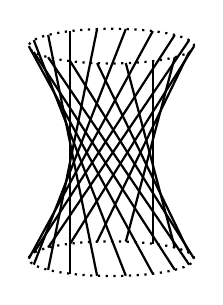
\begin{tikzpicture}[scale=1.0,line width=0.8pt]
  \draw[dotted] (0,1.35) ellipse (1.05 and 0.22);
  \draw[dotted] (0,-1.35) ellipse (1.05 and 0.22);
  \foreach \t in {0,20,...,340}
    \draw ({1.05*cos(\t)},{1.35+0.22*sin(\t)}) -- ({1.05*cos(\t+120)},{-1.35+0.22*sin(\t+120)});
\end{tikzpicture}
\caption{二次曲面 $S:=V(wz-xy)\subset\mathbb{P}^3$ 的两族\trRuling{}之一。一族\trRuling{}含有直线 $V(w,x)$，另一族则含有直线 $V(w,y)$。（图中草绘的这张二次曲面其实是 $a^2+b^2=c^2+1$。你能看出为什么它是 $S$ 的一个\trAffine\trCoordinatePatch{}吗？用 $w$、$x$、$y$、$z$ 来表示，$a$、$b$、$c$ 各是什么？提示：\mbox{练习~5.4.J}。）（依原书手绘图重绘。）}\label{fig:ruling-quadric-surface}
\end{figure}

于是，借助\mbox{练习~5.4.J}，若我们在\trCharacteristic{}不为 $2$ 的\trAlgClosedField{}上工作，我们便已证明：一切秩为 $4$ 的二次曲面都有两族由直线组成的\trRuling。（在\mbox{例~10.6.2}中，我们将认出这个二次曲面就是 $\mathbb{P}^1\times\mathbb{P}^1$。）

\textbf{9.3.10.}\ \emph{旁注：二次超曲面上的\trRuling。}\quad 这两族\trRuling{}的存在性，是好几个重要而美妙的故事共同的第一章。第二章则往往是下面这个。若 $k$ 是\trAlgClosedField，则维数 $m$ 的极大秩（\mbox{练习~5.4.J}）二次超曲面 $X$ 不含维数大于 $m/2$ 的\trLinearSpace{}。（我们将在\mbox{练习~13.3.D}中看到：极大秩的二次超曲面正是「光滑的」二次超曲面。）若 $m=2a+1$，则 $X$ 含有一个不可约的 $\binom{a+2}{2}$ 维的 $a$-平面族。若 $m=2a$，则 $X$ 含有两个不可约的 $\binom{a+1}{2}$ 维的 $a$-平面族；而且，两个 $a$-平面 $\Lambda$ 与 $\Lambda'$ 属于同一族，当且仅当 $\dim(\Lambda\cap\Lambda')\equiv a\pmod 2$。这些\trLinearSpace{}族也称为\trRuling。（欲知更多，可参 [GH1, \S6.1, p.~735, Prop.]。以你现有的知识，已足以想通 $m=0$、$1$、$2$ 的那些例子。$m=2$ 的情形——二次曲面上的\trRuling——将出现在\cref{thm:quadric-cone-section-example}、图~\ref{fig:ruling-quadric-surface}、\mbox{练习~9.3.L}、\S10.6.2、\S12.2.19、\S13.2.12、\mbox{练习~15.5.Q}与\mbox{练习~19.10.M}之中。$m=3$ 的情形则在\mbox{练习~16.4.K}中讨论。）

\textbf{9.3.11.\ \trAffine\trCone{}与\trProjective\trCone{}（图~\ref{fig:cones-of-proj}）。}\quad 若 $S_\bullet$ 是一个\trFinitelyGenerated\trGradedRing，则 $\Proj S_\bullet$ 的\trAffine\trCone{}是 $\Spec S_\bullet$。（警告：这一术语并不理想，因为这个构造依赖于 $S_\bullet$，而不只依赖于 $\Proj S_\bullet$。）作为动机，考察分次环 $S_\bullet=\mathbb{C}[x,y,z]/(z^2-x^2-y^2)$。图~\ref{fig:traditional-cone}是 $\Spec S_\bullet$ 的一幅草图。（这里我们画的是 $z^2=x^2+y^2$ 在 $\mathbb{R}^3$ 中的「实图像」。）它是传统意义上的一个\trCone；原点 $(0,0,0)$ 便是「锥点」。

这给出了一种设想 $\Proj$ 的有用方式（甚至在任意\trRing{}上都行，不限于 $\mathbb{C}$）。直观上，你可以想象：若把原点扔掉，得到的东西便可以投射到 $\Proj S_\bullet$ 上。下面的练习将把这件事说精确。

\begin{figure}[htbp]
\centering
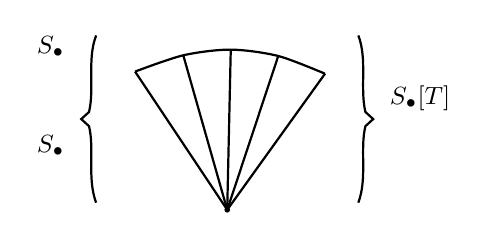
\begin{tikzpicture}[scale=0.9,line width=0.8pt,every node/.style={font=\small}]
  \fill (0,0) circle (0.04);
  \draw plot [smooth] coordinates {(-1.30,1.95) (-0.62,2.18) (0.05,2.26) (0.72,2.17) (1.38,1.92)};
  \draw (0,0) -- (-1.30,1.95);
  \draw (0,0) -- (-0.62,2.18);
  \draw (0,0) -- (0.05,2.26);
  \draw (0,0) -- (0.72,2.17);
  \draw (0,0) -- (1.38,1.92);
  \draw
    (-1.85,0.10)
    .. controls (-1.98,0.45) and (-1.87,0.85) .. (-1.95,1.18)
    -- (-2.06,1.28) -- (-1.95,1.38)
    .. controls (-1.87,1.72) and (-1.98,2.12) .. (-1.85,2.46);
  \draw
    (1.85,0.10)
    .. controls (1.98,0.45) and (1.87,0.85) .. (1.95,1.18)
    -- (2.06,1.28) -- (1.95,1.38)
    .. controls (1.87,1.72) and (1.98,2.12) .. (1.85,2.46);
  \node[anchor=east] at (-2.15,2.30) {$\Proj S_\bullet$};
  \node[anchor=east,align=right] at (-2.15,1.00) {\trAffine\trCone\\ $\Spec S_\bullet$};
  \node[anchor=west,align=left] at (2.15,1.65) {\trProjective\trCone\\ $\Proj S_\bullet[T]$};
\end{tikzpicture}
\caption{$\Proj S_\bullet$ 的\trAffine\trCone{}与\trProjective\trCone{}。（依原书手绘图重绘。）}\label{fig:cones-of-proj}
\end{figure}

\textbf{9.3.M.（练习）}\quad 若 $\Proj S_\bullet$ 是\trField{} $k$ 上的一个\trProjectiveScheme，请描述一个自然的\trMorphism{} $\Spec S_\bullet\setminus V(S_+)\to\Proj S_\bullet$。（你能看出为什么 $V(S_+)$ 恰是一个点、因而理直气壮地该被称作「原点」吗？）

这可以径直推广成下面这道练习，而它又再次为\trIrrelevantIdeal{}这一命名提供了动机。

\textbf{9.3.N.（容易的练习）}\quad 若 $S_\bullet$ 是\trBaseRing{} $A$ 上一个有限生成的\trGradedRing，请描述一个自然的\trMorphism{} $\Spec S_\bullet\setminus V(S_+)\to\Proj S_\bullet$。

事实上，人们可以把这件事说得精确：$\Proj S_\bullet$ 就是仿射锥去掉原点之后，对标量所成的\trMultiplicativeGroup{}取\trQuotient{}的结果。

\textbf{9.3.12.}\ \emph{\trhDefinition{}。}\quad $\Proj S_\bullet$ 的\trProjective\trCone{}是 $\Proj S_\bullet[T]$，其中 $T$ 是一个次数为 $1$ 的新变量。例如，对应于\trConic{} $\Proj k[x,y,z]/(z^2-x^2-y^2)$ 的那个锥，就是 $\Proj k[x,y,z,T]/(z^2-x^2-y^2)$。\trProjective\trCone{}有时也称为 $\Spec S_\bullet$ 的\textbf{\trProjectiveCompletion{}}（projective completion）。（注：这依赖于 $S_\bullet$，而不只是依赖于 $\Proj S_\bullet$。）

\textbf{9.3.O.（不太重要的练习；参看 \S4.5.1）}\quad 证明：$\Proj S_\bullet$ 的「射影锥」$\Proj S_\bullet[T]$ 有一个\trIsomorphic{}于 $\Proj S_\bullet$ 的\trClosedSubscheme（非正式地说，对应于 $T=0$），而其\trComplement{}（即特异开集 $D(T)$）则\trIsomorphic{}于\trAffine\trCone{} $\Spec S_\bullet$。

把这个构造设想为「仿射锥再并上一些『无穷远处』的点」会很有用，而无穷远处的那些点恰好构成这个 $\Proj$。（读者不妨先从图~\ref{fig:traditional-cone}出发，试着把「无穷远处」的那条\trConic{}想象出来，再把这幅想象与图~\ref{fig:affine-projective-cone}相对照。）

至此，我们已把 \S4.5.1 那幅经典图像的代数类比完整地描述了出来。

\textbf{9.3.13.}\ \emph{\trhDefinition{}。}\quad 若我们给 $k[x_0,\dots,x_n]$ 的诸变量配上一组非标准的权——比如说，给 $x_i$ 赋次数 $d_i$——则 $\Proj k[x_0,\dots,x_n]$ 称为\textbf{\trWeightedProjectiveSpace{}}（weighted projective space）$\mathbb{P}(d_0,d_1,\dots,d_n)$。

\textbf{9.3.P.（练习）}\quad
\begin{enumerate}[label=(\alph*)]
  \item 证明：$\mathbb{P}(m,n)$ \trIsomorphic{}于 $\mathbb{P}^1$。
  \item 证明：$\mathbb{P}(1,1,2)\cong\Proj k[u,v,w,z]/(uw-v^2)$。提示：考察 $k[x_0,x_1,x_2]$ 的偶分次部分来做；参\mbox{练习~7.4.D}。（这是一个\trConic{}上的\trProjective\trCone。在\trCharacteristic{}不为 $2$ 的\trField{}上，它\trIsomorphic{}于 $\mathbb{P}^3$ 中传统的锥面 $x^2+y^2=z^2$；见图~\ref{fig:traditional-cone}。）
\end{enumerate}

\begin{figure}[htbp]
\centering
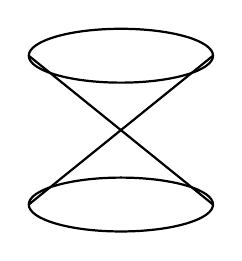
\begin{tikzpicture}[scale=0.9,line width=0.8pt]
  \draw (0,1.05) ellipse (1.30 and 0.38);
  \draw (0,-1.05) ellipse (1.30 and 0.38);
  \draw (-1.30,1.05) -- (1.30,-1.05);
  \draw (1.30,1.05) -- (-1.30,-1.05);
\end{tikzpicture}
\caption{$\mathbb{A}^3$ 中的\trCone{} $x^2+y^2=z^2$。（依原书手绘图重绘。）}\label{fig:traditional-cone}
\end{figure}

\textbf{9.3.Q.（练习：综合运用上面的若干概念）}\quad 证明：$\mathbb{P}(1,1,n)$ \trIsomorphic{}于 $n$ 次\trRationalNormalCurve{}上的\trProjective\trCone。


\section{（闭子）\trSchemeTheoreticImage{}}

我们现在要定义一连串的观念，它们全都属于「使某事成立的最小\trClosedSubscheme」这一形式。其中一例便是局部闭嵌入的\trSchemeTheoretic\trClosure{}这一观念，它将使我们能以三种等价的方式解读局部闭嵌入（\trOpenSubscheme{}交\trClosedSubscheme；\trClosedSubscheme{}的\trOpenSubscheme；\trOpenSubscheme{}的\trClosedSubscheme——参\mbox{练习~9.2.C}）。

\textbf{9.4.1.\ \trSchemeTheoretic\trImage{}（scheme-theoretic image）。}\quad 我们从\trSchemeTheoreticImage{}这个观念谈起。集合论像（set-theoretic image）在一般情形下表现得很糟（\S8.4.1）；即便配上了合理的假设——比如\trChevalley{}定理~8.4.2 中的那些假设——事情仍可能令人迷惑。例如，对于由 $(x,y)\mapsto(x,xy)$ 给出的态射 $\mathbb{A}^2_k\to\mathbb{A}^2_k$，就没有什么合理的办法在其像上安放一个概形结构。定义靶概形的一个\trClosedSubscheme{}——它「最佳逼近」这个像——将会很有用（例如\mbox{练习~9.4.C}）。这将把下面这件事涵括进来：带有非\trReduced{}结构（「\trFuzz」）的对象，其像也可以带有非\trReduced{}结构。照例，我们仍需施加合理的假设，才能让这个观念表现良好（见定理~9.4.4 与推论~9.4.5）。

\textbf{9.4.2.}\ \emph{\trhDefinition{}。}\quad 设 $i\colon Z\hookrightarrow Y$ 是一个\trClosedSubscheme，它给出正合列 $0\to\scr{I}_{Z/Y}\to\OO_Y\to i_*\OO_Z\to 0$。若复合 $\scr{I}_{Z/Y}\to\OO_Y\to\pi_*\OO_X$ 为零，我们就称\textbf{$\pi\colon X\to Y$ 的像落于 $Z$ 中}（the image of $\pi\colon X\to Y$ lies in $Z$）。非正式地说：在局部上，在 $Z$ 上消失的函数\trPullback{}到 $X$ 上就是零函数。若 $\pi$ 的像落于某些子概形 $Z_j$ 之中（$j$ 跑遍某个指标集），则显然它也落于它们的交之中（参\cref{ex:scheme-theoretic-union-intersection}(a)中关于\trClosedSubscheme{}之交的讨论）。我们于是把\textbf{$\pi$ 的\trSchemeTheoretic\trImage{}}——$Y$ 的一个\trClosedSubscheme——定义为「包含该像的最小\trClosedSubscheme」，也就是说，一切包含该像的\trClosedSubscheme{}之交。特别地（在我们最初的几个例子中也是如此），若 $Y$\trAffine，则\trSchemeTheoreticImage{}由 $Y$ 上那些\trPullback{}到 $X$ 上为零的函数切出。

这个概念的其他合理名字还有\emph{闭子\trSchemeTheoreticImage{}}（closed subscheme-theoretic image）或\emph{像闭子概形}（image closed subscheme）。它们的长处在于提醒读者：\trSchemeTheoreticImage{}是一个\emph{闭的}\trSubscheme；但我们不用这些说法。

\emph{\trhExample{}~1.}\quad 考察 $\pi\colon\Spec k[\epsilon]/(\epsilon^2)\to\Spec k[x]=\mathbb{A}^1_k$，由 $x\mapsto\epsilon$ 给出。那么 $\pi$ 的\trSchemeTheoreticImage{}由 $\Spec k[x]/(x^2)$ 给出（\trPullback{}为零的多项式恰是 $x^2$ 的倍式）。可见，这个\trFuzz{}点的像仍带着些许绒毛。

\emph{\trhExample{}~2.}\quad 考察 $\pi\colon\Spec k[\epsilon]/(\epsilon^2)\to\Spec k[x]=\mathbb{A}^1_k$，由 $x\mapsto 0$ 给出。此时\trSchemeTheoreticImage{}由 $\Spec k[x]/(x)$ 给出：像是\trReduced{}的。在这幅图景里，绒毛被 $\pi$「压塌」了。

\emph{\trhExample{}~3.}\quad 考察 $\pi\colon\Spec k[t,t^{-1}]=\mathbb{A}^1-\{0\}\to\mathbb{A}^1=\Spec k[u]$，由 $u\mapsto t$ 给出。任何作为 $t$ 的函数\trPullback{}为零的函数 $g(u)$ 都必是零函数。于是\trSchemeTheoreticImage{}是全空间。而集合论像，另一方面，则是\trDistinguishedOpen{} $\mathbb{A}^1\setminus\{0\}$。由此可见，在不那么病态的情形下，\trSchemeTheoreticImage{}的\trUnderlyingSet{}也可能不是集合论像。但局面还不算糟：\trSchemeTheoreticImage{}的\trUnderlyingSet{}必为\trClosedSet，而且它正是集合论像的\trClosure。我们或许会指望：在合理的情形下这件事总是对的；而在更好的情形下，\trSchemeTheoreticImage{}的\trUnderlyingSet{}就等于集合论像。我们稍后会看到，事实确实如此（\S9.4.6）。

但遗憾的是，病理有时确会现身——嗯，在病态的情势里。

\emph{\trhExample{}~4（图~\ref{fig:yuck-fuzzy-point-image}）。}\quad 令 $X=\bigsqcup_n\Spec k[\epsilon_n]/((\epsilon_n)^n)$（这道概形曾在\mbox{练习~5.2.F}的提示中登场），$Y=\Spec k[x]$，并定义 $X\to Y$：在 $X$ 的第 $n$ 个分支上取 $x\mapsto\epsilon_n$。若 $Y$ 上的函数 $g(x)$ \trPullback{}到 $X$ 上为零，则它的\trTaylor{}展开对一切 $n$ 都到 $n$ 阶为止为零（逐一考察拉回到 $X$ 第 $n$ 个分支上的结果即可），故 $g(x)$ 必为 $0$。（这个论证将在\mbox{练习~13.9.A}(b)中被极大地推广。）于是\trSchemeTheoreticImage{}是 $Y$ 上的 $V(0)$，即 $Y$ 自身；而集合论像则容易看出恰是原点（\trClosedPoint{} $0$）。（这个态射将在警示/例~9.4.11 中隐然现身。）

\begin{figure}[htbp]
\centering
\begin{tikzpicture}[scale=1.0,line width=0.8pt]
  \node at (0,2.75) {$\vdots$};
  \draw[dashed] (-0.55,2.05) -- (0.55,2.05);
  \fill (0,2.05) circle (0.05);
  \draw[dashed] (-0.42,1.62) -- (0.42,1.62);
  \fill (0,1.62) circle (0.05);
  \draw[dashed] (-0.30,1.24) -- (0.30,1.24);
  \fill (0,1.24) circle (0.05);
  \fill (0,0.78) circle (0.055);
  \draw[gray!75,->] (0,0.45) -- (0,-0.95);
  \draw (-1.7,-1.15) -- (1.7,-1.15);
  \node[anchor=west] at (0.85,1.85) {$X$};
  \node[anchor=west] at (1.95,-1.15) {$Y$};
\end{tikzpicture}
\caption{真恶心（定义~9.4.2 的例~4）。（依原书手绘图重绘。）}\label{fig:yuck-fuzzy-point-image}
\end{figure}

\textbf{9.4.3.\ 计算\trSchemeTheoreticImage{}的仿射局部判据。}\quad 不过例~4 显然很怪异；我们可以证明：在「合理的情势」下，这种病理并不会出现。

在靶 $Y$ \trAffine{}的特殊情形（请留意这一论证在例~1 至例~3 中是如何运作的），比如说 $Y=\Spec B$，几乎按定义，$\pi\colon X\to Y$ 的\trSchemeTheoreticImage{}就由理想 $I\subset B$——$Y$ 上那些\trPullback{}到 $X$ 上为零的函数——切出。

若能用这一点对\trSchemeTheoreticImage{}逐片仿射（仿射局部地）进行计算，那就太好了。在\trAffine\trOpenSet{} $\Spec B\subset Y$ 上，定义 $B$ 中由那些\trPullback{}到 $X$ 上为 $0$ 的函数组成的理想 $I(B)\subset B$。形式化地，$I(B):=\ker\bigl(B\to\Gamma(\Spec B,\pi_*\OO_X)\bigr)$。若对每个这样的 $B$ 及每个 $g\in B$，映射 $\varphi\colon I(B)_g\to I(B_g)$ 都是\trIsomorphism，则我们便把\trSchemeTheoreticImage{}定义成了一个\trClosedSubscheme（见\mbox{练习~9.1.F}）。$\varphi$ 的单射性是直截了当的：若 $r\in B$ 而 $r/g^n$ 拉回到 $\pi^{-1}(\Spec B_g)$ 上为零，则由于 $g$ 在 $\Spec B_g=D(g)$ 的所有点处都不消失，$\pi^\sharp(r)$ 在 $\pi^{-1}(\Spec B_g)$ 上也为零。

于是问题便是 $\varphi$ 的满射性；把它翻译过来就是：给定 $D(g)$ 上一个拉回到 $\pi^{-1}(D(g))$ 上为零的函数 $r/g^n$，是否对某个 $m$ 有 $rg^m$ 拉回到 $\pi^{-1}(\Spec B)$ 上为零？

（i）我们先来证明：若 $\pi^{-1}(\Spec B)$\trReduced，则答案是肯定的。此时我们可以利用\mbox{练习~5.2.A}：\trReduced\trScheme{}上的函数，只要在每一点处的取值都为零，就为零。于是我们可以取 $m=1$（因为 $\pi^\sharp(r)$ 在 $\pi^{-1}(D(g))$ 上消失，而 $g$ 在 $V(g)$ 上消失，故 $\pi^\sharp(rg)$ 在 $\pi^{-1}(\Spec B)=\pi^{-1}(D(g))\cup\pi^{-1}(V(g))$ 上消失）。

（ii）若 $\pi^{-1}(\Spec B)$\trAffine，比如说为 $\Spec A$，答案也是肯定的：设 $r'=\pi^\sharp(r)$、$g'=\pi^\sharp(g)$ 落在 $A$ 中；若 $r'$ 在 $D(g')$ 上为零，则存在 $m$ 使 $r'(g')^m=0$（「$r'$ 在 $D(g')$ 上为零」这句话的含义恰恰就是这个——$D(g')$ 上的函数正是 $A_{g'}$）。

（ii）$'$ 更一般地，若 $\pi^{-1}(\Spec B)$\trQuasicompact，答案也是肯定的：用有限多个\trAffine\trOpenSet{}覆盖 $\pi^{-1}(\Spec B)$。对其中每一个，都会有某个 $m_i$，使 $rg^{m_i}$ 拉回到这个开集上为零。然后取 $m=\max(m_i)$。（我们再次看到：拟紧性是我们的朋友！）

总之，我们证明了下面这条（颇为微妙的）定理。

\textbf{9.4.4.\ \trhTheorem{}。}\ ——\ \emph{设 $\pi\colon X\to Y$ 是概形间的\trMorphism。若 $X$\trReduced{}或 $\pi$\trQuasicompact，则 $\pi$ 的\trSchemeTheoreticImage{}可以仿射局部地计算：在 $\Spec A\subset Y$ 上，它由那些\trPullback{}为函数 $0$（在 $\pi^{-1}(\Spec A)$ 上）的函数（即 $A$ 的元素）切出。}

\textbf{9.4.5.\ \trhCorollary{}。}\ ——\ \emph{在定理~9.4.4 的假设下，$\pi$ 的集合论像的\trClosure{}就是\trSchemeTheoreticImage{}的\trUnderlyingSet。}

（上面的例~4 表明，这些假设是必需的。）

\textbf{9.4.6.}\quad 特别地，若集合论像是闭的（例如 $\pi$\trFinite{}或\trProjective），则集合论像就是\trSchemeTheoreticImage{}的\trUnderlyingSet——正如上面的例~3 所许诺的那样。

\textbf{9.4.7.}\ \emph{\trhCorollary{}~9.4.5 的证明。}\quad 集合论像含于\trSchemeTheoreticImage{}的\trUnderlyingSet{}之中。（请自行检验！）\trSchemeTheoreticImage{}的\trUnderlyingSet{}是闭集，故集合论像的\trClosure{}含于\trSchemeTheoreticImage{}的\trUnderlyingSet{}之中。另一方面，若 $U$ 是集合论像之\trClosure{}的\trComplement，则 $\pi^{-1}(U)=\varnothing$。在这些假设下，\trSchemeTheoreticImage{}可以局部地计算，故在 $U$ 上\trSchemeTheoreticImage{}是空集。\hfill$\square$

我们以几条零散的评注作结。

\textbf{9.4.A.（容易练习）}\quad 若 $X$\trReduced，证明：$\pi\colon X\to Y$ 的\trSchemeTheoreticImage{}也\trReduced。

更一般地，你或许会指望：像上不该有不被源的非\trReduced{}结构所强迫的多余非\trReduced{}结构。下面这条练习在局部\trNoetherian{}的情形（此时我们可以谈论\trAssociatedPoint）把这件事说精确。

\textbf{9.4.B.}\ \hard\ \textbf{（不重要练习）}\quad 若 $\pi\colon X\to Y$ 是局部\trNoetherian{}概形之间的\trQuasicompact\trMorphism，证明：像子概形的诸\trAssociatedPoint{}构成 $X$ 的诸\trAssociatedPoint{}之像的一个子集。（例 $\bigsqcup_{a\in\mathbb{C}}\Spec\mathbb{C}[t]/(t-a)\to\Spec\mathbb{C}[t]$ 表明，若你放弃拟紧性会出什么岔子——注意，源的\trReducedness{}帮不上忙。）提示：化归到 $X$ 与 $Y$ 都\trAffine{}的情形。（你能否培养出一种几何直观，让这件事在你看来是顺理成章的？）

\textbf{9.4.8.\ 局部闭子概形的\trSchemeTheoretic\trClosure。}\quad 我们把局部闭嵌入 $\pi\colon X\hookrightarrow Y$ 的\textbf{\trSchemeTheoretic\trClosure{}}（scheme-theoretic closure）定义为 $\pi$ 的\trSchemeTheoreticImage{}。（一个更简短的说法是 schematic closure（概形闭包），不过这个更雅致的命名并未流行开来。）

\textbf{9.4.C.（练习）}\quad 若局部闭嵌入 $V\hookrightarrow X$ 是\trQuasicompact{}的（例如 $V$ \trNoetherian{}时，\cref{ex:quasicompact-quasiseparated-source}(a)；或 $V$ \trReduced{}时），证明：\mbox{练习~9.2.C}中的 (iii) 蕴含 (i) 与 (ii)。于是，在这一幸运的情势下，局部闭嵌入可以用三种不同的方式来思考，哪种方便用哪种。（提示：推论~9.4.5。）

\textbf{9.4.D.（不重要练习，但有助直观）}\quad 若 $\pi\colon X\hookrightarrow Y$ 是向一个局部\trNoetherian{}概形中的局部闭嵌入（于是 $X$ 也局部\trNoetherian），则\trSchemeTheoretic\trClosure{}的诸\trAssociatedPoint{}（自然地双射于）$X$ 的诸\trAssociatedPoint。（提示：\mbox{练习~9.4.B}。）非正式地说：\trSchemeTheoretic{}闭包上唯一的非\trReduced{}结构，就是被 $X$ 上的非\trReduced{}结构「强迫出来的」那一点。

\textbf{9.4.9.\ 闭子集上的（既约）子概形结构。}\quad 设 $X^{\mathrm{set}}$ 是概形 $Y$ 的一个闭\emph{子集}。那么我们可以在 $X^{\mathrm{set}}$ 上定义一个\trCanonical{}的概形结构 $X$，它是既约的。我们可以把它描述为：由那些在 $X^{\mathrm{set}}$ 的所有点处取值都为零的函数切出。在 $Y$ 的\trAffine\trOpenSet{} $\Spec B$ 上，若集合 $X^{\mathrm{set}}$ 对应于\trRadicalIdeal{} $I=I(X^{\mathrm{set}}\cap\Spec B)$（回想 \S3.7 中的函数 $I(\cdot)$），则概形 $X$ 对应于 $\Spec B/I$。你可以很快核验：这个构造对任何特异包含 $\Spec B_f\hookrightarrow\Spec B$ 都表现良好。我们还可以按下面这种疯狂的方式，把这个构造看作\trSchemeTheoreticImage{}的一例：令 $W$ 是把 $X^{\mathrm{set}}$ 的所有点作成\trDisjointUnion{}所得的概形——对应于 $X^{\mathrm{set}}$ 中点 $p$ 的那个点，就是 $\OO_{Y,p}$ 的\trResidueField{}之谱。令 $\rho\colon W\to Y$ 为「\trCanonical」映射：把「$p$」送到 $p$，并在剩余域上给出\trIsomorphism。那么 $X$ 上的概形结构便是 $\rho$ 的\trSchemeTheoreticImage{}。第三种定义：它是那种\trUnderlyingSet{}包含 $X^{\mathrm{set}}$ 的最小\trClosedSubscheme。

\textbf{9.4.E.（练习）}\quad 证明：这三种定义全都相同。

这个构造称为闭子集 $X^{\mathrm{set}}$ 上的（诱导）\textbf{\trReduced\trSubscheme{}结构}（reduced subscheme structure）。（一道含糊的练习：请把既约子概形结构这个定义弄得精确而严格，直到你自己满意为止。）

\textbf{9.4.F.（练习）}\quad 证明：诱导既约子概形 $X\hookrightarrow Y$ 的\trUnderlyingSet{}确是闭子集 $X^{\mathrm{set}}$。证明：$X$\trReduced。

\textbf{9.4.10.\ 概形的既约版本。}\quad 在最要紧的情形，即 $X^{\mathrm{set}}$ 为整个 $Y$ 时，我们得到一个\emph{\trReduced\trClosedSubscheme} $Y^{\mathrm{red}}\hookrightarrow Y$，称为 $Y$ 的\textbf{\trReduction{}}（reduction）。在\trAffine\trOpenSubset{} $\Spec B\hookrightarrow Y$ 上，$Y^{\mathrm{red}}\hookrightarrow Y$ 对应于（对 $B$ 的\trNilradical{} $\mathfrak{N}(B)$）取商的结果。概形的\trReduction{}就是概形的「既约版本」；非正式地说，它对应于「把绒毛剪掉」。

另一个等价的\trReduction{}定义：在\trAffine\trOpenSubset{} $\Spec B\hookrightarrow Y$ 上，$Y$ 的\trReduction{}对应于\trNilradical{} $\mathfrak{N}(B)\subset B$。我们容易核验：对任意 $f\in B$，$\mathfrak{N}(B)_f=\mathfrak{N}(B_f)$。由\mbox{练习~9.1.F}，这就定义出一个\trClosedSubscheme，我们称之为\trReduction{}。

\textbf{9.4.11.}\ \hard\ \emph{\trhCaveat{}/\trhExample{}。}\quad 下述说法并不成立：对\emph{每个}开子集 $U\subset Y$，$\Gamma(U,\OO_{Y^{\mathrm{red}}})$ 都等于 $\Gamma(U,\OO_Y)$ 模去其幂零元的结果。例如，在 $Y=\bigsqcup_n\Spec k[x]/(x^n)$ 上，函数 $x$ 并不幂零，但它在 $Y^{\mathrm{red}}$ 上为 $0$，因为它是「\trLocally\trNilpotent」的。这或许会让你想起定义~9.4.2 之后的例~4。


\section{用\trEffectiveCartierDivisor{}{}\trSlicing{}、\trRegularSequence{}与\trRegularEmbedding{}}

我们现在引入\trRegularEmbedding{}（regular embedding）——局部闭嵌入中重要的一类。从\trRegular\trScheme{}到\trRegular\trScheme{}之内的局部闭嵌入，便是\trRegularEmbedding{}的一个重要例子（\mbox{练习~13.2.M}(b)）。有效卡蒂耶除子（effective Cartier divisor）——基本上就是余维数 $1$ 的情形——日后也将被一再证明有用；「反复用有效卡蒂耶除子\trSlicing{}」为许多论证提供了归纳步骤。（今后在许多语境下，当我们说\textbf{\trSlicing{}}（slicing）时，指的都是用有效卡蒂耶除子作\trSlicing{}。）

\textbf{9.5.1.\ \trLocallyPrincipal{}闭子概形，与有效卡蒂耶除子。}\quad 一个\trClosedSubscheme{}称为\textbf{\trLocallyPrincipal{}}（locally principal）的，若在足够细的一个\trOpenCover{}的每个\trOpenSet{}上，它都由单个方程切出（也就是说，由一个\trPrincipalIdeal{}切出——术语正由此得名）。更确切地说，\trLocallyPrincipal{}闭子概形是这样的\trClosedSubscheme{} $\pi\colon X\hookrightarrow Y$：存在 $Y$ 的一个\trOpenCover{} $\{U_i\}$，使得对每个 $i$，$\pi^{-1}(U_i)\hookrightarrow U_i$ 都\trIsomorphic{}于某个形如 $V(s_i)\hookrightarrow U_i$ 的\trClosedSubscheme，其中 $s_i\in\Gamma(U_i,\OO_Y)$。（这个\trOpenCover{}显然可以取成由\trAffine\trOpenSubset{}组成的。）

例如，$\mathbb{P}^n_k$ 中的超曲面（定义~9.3.2）就是\trLocallyPrincipal{}的：$n+1$ 个变元之间的每个齐次多项式都定义了 $\mathbb{P}^n_A$ 的一个\trLocallyPrincipal{}闭子概形。（\trhWarning：与「\trLocallyPrincipal{}性」不同，「主性」并不是一个仿射局部条件；见 \S19.11.10！此外，射影超曲面的例子（\S9.3.1）表明：\trLocallyPrincipal{}闭子概形未必由一个整体有定义的函数切出。最后，很遗憾，在 \S15.4.8 中我们会以另一种意思使用「\trLocallyPrincipal{}」这个说法。）

若\trIdealSheaf{}在每一点附近都由一个\trNonZerodivisor{}函数局部生成，我们就称这个闭子概形为一个有效卡蒂耶除子。更确切地说：若 $\pi\colon X\to Y$ 是一个\trClosedEmbedding，且存在由\trAffine\trOpenSubset{} $\Spec A_i\subset Y$ 组成的 $Y$ 的\trCover，并存在\trNonZerodivisor{} $t_i\in A_i$ 使 $V(t_i)=X|_{\Spec A_i}$（在概形论的意义下——也就是说，$X$ 在 $\Spec A_i$ 上的\trIdealSheaf{}由 $t_i$ 生成），那么我们就说 $X$ 是 $Y$ 上的一个\textbf{\trEffectiveCartierDivisor{}{}}。（这个说法的来历我们不作解释，因为它与这里的视角无关。）当我们意指「限制到一个有效卡蒂耶除子上」时，常会用「\textbf{用}一个有效卡蒂耶除子\textbf{\trSlicing{}}」（slicing by an effective Cartier divisor）这个形象的说法。

有效卡蒂耶除子这个观念是核心性的；\trLocallyPrincipal{}闭子概形这个观念则远非如此。

\textbf{9.5.A.（练习）}\quad 设 $t\in A$ 是一个\trNonZerodivisor。证明：对每个\trPrimeIdeal{} $p$，$t$ 在 $A_p$ 中都是\trNonZerodivisor。

\textbf{9.5.2.}\ \emph{\trhCaveat{}。}\quad 若 $D$ 是\trAffineScheme{} $\Spec A$ 上的一个有效卡蒂耶除子，则未必存在 $t\in A$ 使 $D=V(t)$（见\mbox{练习~15.5.I}——\S19.11.10 给出了另一种风味的例子）。换言之，「闭子概形是有效卡蒂耶除子」这一条件可以在\emph{某个}仿射覆盖上得到验证，却不能在\emph{任意}仿射覆盖上检验——它并不是这种显而易见意义上的仿射局部条件。

\textbf{9.5.B.（练习）}\quad 设 $X$ 是一个局部\trNoetherian{}概形。若 $t\in\Gamma(X,\OO_X)$ 是 $X$ 上的一个函数，证明：$t$（或更确切地说，闭子概形 $V(t)$）是一个有效卡蒂耶除子，当且仅当它在 $X$ 的任何\trAssociatedPoint{}上都不消失。证明：$X$ 的一个\trLocallyPrincipal{}闭子概形是有效卡蒂耶除子，当且仅当它不包含 $X$ 的任何\trAssociatedPoint。

\textbf{9.5.C.（练习）}\quad 设 $V(t)=V(t')\hookrightarrow\Spec A$ 是一个有效卡蒂耶除子，其中 $t$ 与 $t'$ 都是 $A$ 中的\trNonZerodivisor。证明：$t$ 是 $t'$ 的可逆函数倍。

有效卡蒂耶除子的想法把我们引向\trRegularSequence（regular sequence）的观念。（我们将在\mbox{练习~9.5.H}中完成闭环：届时我们将把任何合理概形上的有效卡蒂耶除子解读为余维数 $1$ 的\trRegularEmbedding{}。）

\textbf{9.5.3.\ \trRegularSequence{}。}\quad 「正则序列」这个观念——如同其他许多观念一样——归功于\trSerre{}[Se2]。正则序列的定义，是下述几何想法的代数版本：局部地，我们取一个有效卡蒂耶除子（一个\trNonZerodivisor）；然后再取其上的一个有效卡蒂耶除子；然后再取其上的一个有效卡蒂耶除子；如此进行，做有限多次。这里需要一点小心；比如说，我们可能希望这件事与所加方程的次序无关，而只有在我们把这话说对的时候，这才是真的。

我们对环 $A$ 给出\trRegularSequence{}的定义，并对 $A$-\trModule{} $M$ 作更一般的叙述。

\textbf{9.5.4.}\ \emph{\trhDefinition{}。}\quad 若 $M$ 是一个 $A$-\trModule，则 $A$ 中元素组成的序列 $x_1,\dots,x_r$ 称为一条\textbf{$M$-\trRegularSequence}（$M$-regular sequence；或\textbf{对 $M$ 的\trRegularSequence}，regular sequence for $M$），若下述两个条件得到满足。
\begin{enumerate}[label=(\roman*)]
\item 对每个 $i$，$x_i$ 都不是 $M/(x_1,\dots,x_{i-1})M$ 的\trZerodivisor。（$i=1$ 的情形应解读为：「$x_1$ 不是 $M$ 的\trZerodivisor」。回想：\trZerodivisor{}定义于\cref{ex:when-localization-is-injective}。）
\item 我们有真包含 $(x_1,\dots,x_r)M\subsetneq M$。
\end{enumerate}

在我们最关心的情形 $M=A$ 中，这应当被看作「\trCompleteIntersection」（complete intersection）的一个合理近似；而且事实上我们就将把它当作定义来使用（\S9.5.7）。

对\trRegularSequence{} $x_1,\dots,x_r\in A$，我们称 $r$ 为\textbf{\trRegularSequence{}的\trLength}。一条 $A$-\trRegularSequence{}就径直称为\textbf{\trRegularSequence}。

\textbf{9.5.D.（练习）}\quad 若 $M$ 是一个 $A$-\trModule，证明：一条 $M$-\trRegularSequence{}在任何局部化之后，仍满足\trRegularSequence{}的定义~9.5.4 中的条件 (i)。（等你懂得了何为\trFlatness{}之后，你将会看到：你的论证恰恰表明条件 (i) 在任何平坦\trBaseChange{}下保持。）

\textbf{9.5.E.（练习）}\quad 若 $x,y$ 是一条 $M$-\trRegularSequence，证明：$x^N,y$ 也是一条 $M$-\trRegularSequence。提示：困难的部分在于证明 $y$ 不是 $M/(x^N M)$ 的\trZerodivisor。请对 $N$ 作归纳来证明这一点。若 $y$ 是 $M/(x^N M)$ 的\trZerodivisor，则对某个 $m\in M\setminus x^N M$ 有 $ym\equiv 0\pmod{x^N}$。于是 $ym=x^N k$，其中 $k\in M$。利用「$x,y$ 是一条\trRegularSequence」这一事实，证明 $m$ 是 $x$ 的倍数。（你的论证将可以轻易推广，从而更一般地证明：若 $x_1,\dots,x_n$ 是一条\trRegularSequence，而 $a_1,\dots,a_n\in\mathbb{Z}^+$，则 $x_1^{a_1},\dots,x_n^{a_n}$ 是一条\trRegularSequence。）

\textbf{9.5.5.}\ \emph{序列的正则性依赖于其次序。}\quad 我们现在给出一个例子（[E, Example 17.3]），表明\trRegularSequence{}的次序是有关系的。设 $A=k[x,y,z]/(x-1)z$，于是 $X=\Spec A$ 是平面 $z=0$ 与平面 $x=1$ 之并——$X$\trReduced，且有两个\trIrreducibleComponent（见图~\ref{fig:regular-sequence-order}）。你可以轻而易举地核验：$x$ 是 $A$ 的\trNonZerodivisor（$x=0$ 错过 $X$ 的一个\trIrreducibleComponent，而在另一个上也不完全消失），并且相应的有效卡蒂耶除子 $X'=\Spec k[x,y,z]/(x,z)$（在 $X$ 上）是\trIntegral{}的。于是 $(x-1)y$ 给出 $X'$ 上的一个有效卡蒂耶除子（它在 $X'$ 上不完全消失），故 $x,(x-1)y$ 是 $A$ 的一条正则序列。然而，$(x-1)y$ 并\emph{不}是 $A$ 的\trNonZerodivisor，因为它\emph{确实}在两个\trIrreducibleComponent{}之一上完全消失。于是 $(x-1)y,x$ 就\emph{不}是正则序列。重排\trRegularSequence{} $x,(x-1)y$ 会毁掉正则性，其缘由是清楚的：存在一个\trLocus，在其上 $(x-1)y$ 并非有效卡蒂耶；但若我们先强加 $x=0$，它就不见了。这里的问题是一种「非局部性」——在「$x=y=z=0$ 附近」根本没有问题。这或许可以让我们预感到：在（\trNoetherian{}的）局部情势下，这个问题会消失。我们现在把这件事说精确。

\textbf{9.5.6.\ \trhTheorem{}。}\ ——\ \emph{设 $(A,\mathfrak{m})$ 是一个\trNoetherian{}\trLocalRing，$M$ 是一个有限生成的 $A$-\trModule。那么含于 $\mathfrak{m}$ 中的任何 $M$-\trRegularSequence{} $(x_1,\dots,x_r)$ 在任何重排之下仍是\trRegularSequence。}

（在 [Di] 中，\trDieudonne{}给出了一个占半页的例子，表明\trNoetherian{}假设在定理~9.5.6 中是必需的。此外，在\mbox{练习~24.6.C}中，当 $A$ 包含一个域时，我们给出了一个不同的、多少要简单些的证明。）

在证明定理~9.5.6 之前（证明见于\mbox{练习~9.5.F}），我们先证第一个非平凡情形，即 $r=2$ 的情形。这段讨论暗地里是 Koszul 复形（Koszul complex）的一个婴孩情形（\S24.4.1 将简要提到这个复形）。

\begin{figure}[htbp]
\centering
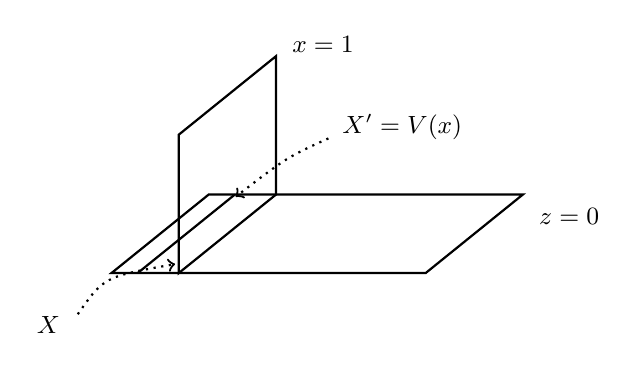
\begin{tikzpicture}[scale=0.95,line width=0.8pt,every node/.style={font=\small}]
  \draw (0,0) -- (4.2,0) -- (5.5,1.05) -- (1.3,1.05) -- cycle;
  \draw (0.35,0) -- (1.65,1.05);
  \draw (0.9,0) -- (2.2,1.05) -- (2.2,2.9) -- (0.9,1.85) -- cycle;
  \node[anchor=west] at (2.28,3.05) {$x=1$};
  \node[anchor=west] at (5.58,0.75) {$z=0$};
  \node[anchor=west] at (2.95,1.95) {$X' = V(x)$};
  \draw[dotted,->] (2.9,1.8) .. controls (2.35,1.55) .. (1.66,1.02);
  \node[anchor=east] at (-0.55,-0.7) {$X$};
  \draw[dotted,->] (-0.45,-0.55) .. controls (-0.1,-0.05) .. (0.85,0.12);
\end{tikzpicture}
\caption{\trRegularSequence{}中次序有关系（在「非局部」的情势下），理由毫不令人惊讶。（依原书手绘图重绘。）}\label{fig:regular-sequence-order}
\end{figure}

设 $\mathfrak{m}$ 中的元素 $x$ 与 $y$ 组成一条 $M$-\trRegularSequence。翻译过来就是：$x\in\mathfrak{m}$ 在 $M$ 上是\trNonZerodivisor，而 $y\in\mathfrak{m}$ 在 $M/xM$ 上是\trNonZerodivisor。

考察\trDoubleComplex
\begin{equation*}\tag{9.5.6.1}\label{eq:double-complex-regular-sequence}
\begin{tikzcd}[row sep=3em, column sep=4.2em]
M \ar[r, "\times(-x)"] & M \\
M \ar[u, "\times y"] \ar[r, "\times x"] & M, \ar[u, "\times y"]
\end{tikzcd}
\end{equation*}
其中左下角被认为处于位置 $(0,0)$。（上一行出现负号的唯一理由，是我们在 \S1.6.1 中偏爱反交换方块而非交换方块的任意口味；但它实在无关紧要。）

我们用一条（简单的）\trSpectralSequence{}来计算\trTotalComplex{}的\trCohomology，从右行定向开始。（在这里动用谱序列——正如在我们其他许多应用中那样——实属大材小用；我们这么做，部分是为了练一练这台机器。）在第一\trPage，我们有
\begin{equation*}\tag{9.5.6.2}\label{eq:regular-sequence-first-page}
\begin{tikzcd}[row sep=3.2em, column sep=4.5em]
\ker\bigl(M\mathrel{\xrightarrow{\ \times x\ }}M\bigr) & M/xM \\
\ker\bigl(M\mathrel{\xrightarrow{\ \times x\ }}M\bigr) \ar[u, "\times y"] & M/xM. \ar[u, "\times y"]
\end{tikzcd}
\end{equation*}
第一列中的诸 $\ker\bigl(M\mathrel{\xrightarrow{\ \times x\ }}M\bigr)$ 都是 $0$，因为 $x$ 在 $M$ 上是\trNonZerodivisor。在竖直方向取\trHomology{}以得到第二\trPage，我们发现
\begin{equation*}\tag{9.5.6.3}\label{eq:regular-sequence-second-page}
\begin{array}{c@{\qquad}c}
0 & M/(x,y)M\\[0.8em]
0 & 0,
\end{array}
\end{equation*}
这里用到了 $y$ 在 $M/xM$ 上是\trNonZerodivisor{}这一事实。该\trSpectralSequence{}显然在此处\trConverge。于是，原来的\trDoubleComplex{} \eqref{eq:double-complex-regular-sequence} 只在次数 $2$ 处有非零\trCohomology，且在该处\trCohomology{}为 $M/(x,y)M$。

现在我们改用上行定向对 \eqref{eq:double-complex-regular-sequence} 跑一遍\trSpectralSequence。这条\trSpectralSequence{}的第一\trPage{}为：
\[
\begin{tikzcd}[row sep=4.6em, column sep=5.5em]
M/yM \ar[r, "\times(-x)"] & M/yM \\
\ker\bigl(M\mathrel{\xrightarrow{\ \times y\ }}M\bigr) \ar[r, "\times x"] & \ker\bigl(M\mathrel{\xrightarrow{\ \times y\ }}M\bigr).
\end{tikzcd}
\]
该\trSpectralSequence{}在下一步之后必定\trConverge{}到 \eqref{eq:regular-sequence-second-page}。从上一行可以看出：乘 $x$ 在 $M/yM$ 上必定是单射，故 $x$ 在 $M/yM$ 上是\trNonZerodivisor。从下一行可以看出：乘 $x$ 给出 $\ker\bigl(M\mathrel{\xrightarrow{\ \times y\ }}M\bigr)$ 与自身之间的一个\trIsomorphism。由于 $x\in\mathfrak{m}$，据\trNakayama{}引理版本~2（引理~8.2.9），这就蕴含 $\ker\bigl(M\mathrel{\xrightarrow{\ \times y\ }}M\bigr)=0$，故 $y$ 在 $M$ 上是\trNonZerodivisor。于是我们便证明了：$y,x$ 构成 $M$ 上的一条\trRegularSequence——这正是定理~9.5.6 的 $r=2$ 情形。

\textbf{9.5.F.（容易练习）}\quad 证明定理~9.5.6。（提示：先证只交换两个相邻 $x_i$ 的那种重排，用刚才讨论的 $r=2$ 情形。）\trNoetherian{}假设都是在哪些地方被用到的？

\textbf{9.5.7.\ \trRegularEmbedding{}。}\quad 设 $\pi\colon X\hookrightarrow Y$ 是一个局部闭嵌入。我们说 $\pi$ \textbf{在点 $p\in X$ 处是（余维数 $r$ 的）\trRegularEmbedding{}}（regular embedding (of codimension $r$) at a point），若在\trLocalRing{} $\OO_{Y,p}$ 中，$X$ 的\trIdeal{}由一条（长度为 $r$ 的）\trRegularSequence{}生成。我们说 $\pi$ 是一个\textbf{（余维数 $r$ 的）\trRegularEmbedding{}}，若它在所有 $p\in X$ 处都是（余维数 $r$ 的）\trRegularEmbedding{}。（\trRegularEmbedding{}的另一个合理的名字本来可以是「局部完全相交」（local complete intersection）。不幸的是，「局部完全相交态射」（local complete intersection morphism），或「lci 态射」（lci morphism），已被用来指另一个相关的观念；见 [Stacks, tag 068E]。）

我们的术语用到了「余维数」这个词，而我们尚未把这个词单独当作一个词来定义。使用这个词的理由，在你见到\trKrull{}主理想定理~12.3.3 与\trKrull{}高度定理~12.3.10 之后，会变得更清楚。

\textbf{9.5.G.（练习：局部闭嵌入为\trRegularEmbedding{}这一条件是开的）}\quad 证明：若局部\trNoetherian{}概形之间的局部闭嵌入 $\pi\colon X\hookrightarrow Y$ 在 $p$ 处是\trRegularEmbedding{}，则它在 $X$ 中 $p$ 的某个\trOpen\trNeighborhood{}上都是\trRegularEmbedding{}。提示：先化归到 $\pi$ 是闭嵌入的情形，再化归到 $Y$（从而 $X$）仿射的情形——比如说 $Y=\Spec B$、$X=\Spec B/I$、$p=[p]$——并且存在 $f_1,\dots,f_r$，使得在 $\OO_{Y,p}$ 中诸 $f_i$ 的像组成一条生成 $I_p$ 的正则序列。我们希望证明：在「$p$ 的某个\trOpen\trNeighborhood{}中」有 $(f_1,\dots,f_r)=I$。请证明下述代数事实：若 $I$ 与 $J$ 是\trNoetherian{}环 $A$ 的两个\trIdeal，而 $p\subset A$ 是满足 $I_p=J_p$ 的一个\trPrimeIdeal，则存在 $a\in A\setminus p$ 使得在 $A_a$ 中 $I_a=J_a$。为证此，请先证明只需考虑 $I\subset J$ 这一特殊情形——做法是改考虑 $I\cap J$ 与 $J$。为证这一特殊情形，令 $K=J/I$（一个有限生成的\trModule），并证明：若 $K_p=0$，则对某个 $a\in A\setminus p$ 有 $K_a=0$。

于是，若 $X$ 在一个域上\trLocally\trFiniteType（例如是一个\trVariety），则要检验一个闭嵌入 $\pi$ 是不是\trRegularEmbedding{}，只需在 $X$ 的诸\trClosedPoint{}处检验就够了（\mbox{练习~5.3.F}）。

\mbox{练习~13.1.F}(b) 将证明：并非所有闭嵌入都是\trRegularEmbedding{}。

\textbf{9.5.H.（练习）}\quad 证明：局部\trNoetherian{}概形的闭嵌入 $X\hookrightarrow Y$ 是余维数 $1$ 的\trRegularEmbedding{}，当且仅当 $X$ 是 $Y$ 上的一个有效卡蒂耶除子。不重要的注记：\trNoetherian{}假设可以换成要求 $\OO_Y$ \trCoh，论证本质上照旧。有意思的是：「有效卡蒂耶除子」永远蕴含「余维数 $1$ 的\trRegularEmbedding{}」，但逆向的论证却需要\trNoetherian（或类似）的假设。（逆向命题的反例见 [MO129242]。）

\textbf{9.5.8.}\ \emph{\trhDefinition{}。}\quad 概形 $Y$ 中的一个\textbf{余维数 $r$ 完全相交}（codimension $r$ complete intersection）是一个闭子概形 $X$：它可以写成 $r$ 个有效卡蒂耶除子 $D_1,\dots,D_r$ 的\trSchemeTheoretic{}交，使得在每一点 $p\in X$ 处，与 $D_1,\dots,D_r$ 相应的方程都组成一条正则序列。\textbf{\trCompleteIntersection{}}这个说法意指「对某个 $r$ 的余维数 $r$ 完全相交」。

